\documentclass[border=5pt]{standalone}
\usepackage{tikz}
\usepackage{tikz-3dplot}
\usetikzlibrary{arrows.meta, 3d, perspective, calc}
\usepackage{amsmath}
\begin{document}
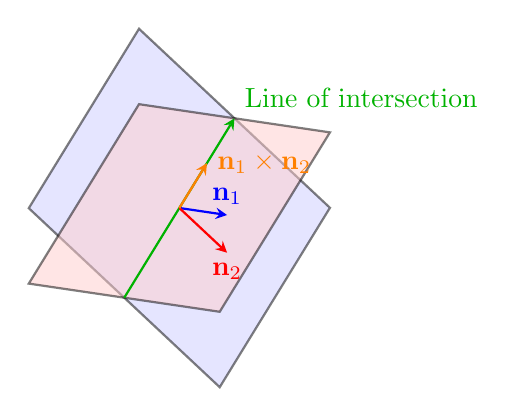
\begin{tikzpicture}[scale=0.7, >=stealth, 3d view={30}{70} ]
    % Draw two planes intersecting
    \draw[thick, fill=blue!20, opacity=0.5]
        (0,0,4) -- (4,0,0) -- (4,4,0) -- (0,4,4) -- cycle;
    \draw[thick, fill=red!20, opacity=0.5]
        (0,0,0) -- (4,0,4) -- (4,4,4) -- (0,4,0) -- cycle;

    % Line of intersection
    \draw[thick, green!70!black, ->] (2,0,2) -- (2,4,2) node[above right] {Line of intersection};

    % Normal vectors to the planes
    \draw[->,thick,blue] (2,2,2) -- ($(2,2,2)+(1,0,1)$) node[above] {$\mathbf{n}_1$};
    \draw[->,thick,red] (2,2,2) -- ($(2,2,2)+(1,0,-1)$) node[below] {$\mathbf{n}_2$};

    % Direction of intersection
    \draw[->,thick,orange] (2,2,2) -- ($(2,2,2)+(0,1,0)$) node[right] {$\mathbf{n}_1 \times \mathbf{n}_2$};

\end{tikzpicture}
\end{document}
